% Chapter 2.11: Processors (3-OS) - LaTeX Beamer Slides
% Structured Computer Architecture: An Order-Based Approach
% Authors: John Glossner and Gheorghe M. Ştefan

\documentclass[aspectratio=169,11pt]{beamer}

% Theme and color scheme (simple, print-friendly)
\usetheme{default}
\usecolortheme{default}

% Simple color scheme for printing
\definecolor{titlecolor}{RGB}{0,0,0}
\definecolor{accentcolor}{RGB}{0,0,139}
\definecolor{textcolor}{RGB}{0,0,0}

% Set colors
\setbeamercolor{title}{fg=titlecolor}
\setbeamercolor{frametitle}{fg=titlecolor}
\setbeamercolor{structure}{fg=accentcolor}
\setbeamercolor{normal text}{fg=textcolor}

% Remove navigation symbols
\setbeamertemplate{navigation symbols}{}

% Simple footline
\setbeamertemplate{footline}[frame number]

% Packages
\usepackage{amsmath}
\usepackage{amsfonts}
\usepackage{amssymb}
\usepackage{graphicx}
\usepackage{tikz}
\usepackage{booktabs}
\usepackage{array}
\usepackage{listings}
\usepackage{xcolor}


% Set graphics path for images (relative to slides directory)
\graphicspath{{../Images/}}

% Title information
\title[Chapter 2.11: Processors]{Structured Computer Architecture\\Chapter 2.11: Processors\\Third-Order Systems (3-OS)}
\subtitle{An Order-Based Approach}
\author{John Glossner and Gheorghe M. Ştefan}
\institute{Based on the textbook}
\date{\today}

% Custom commands
\newcommand{\concept}[1]{\textbf{\color{accentcolor}#1}}
\newcommand{\defterm}[1]{\textit{#1}}

\begin{document}

% Title slide
\begin{frame}
\titlepage
\end{frame}

% Table of contents
\begin{frame}{Outline}
\tableofcontents
\end{frame}

% Learning Objectives
\begin{frame}{Learning Objectives}
By the end of this chapter, you will be able to:
\begin{itemize}
\item Understand third-order systems (3-OS) and the third feedback loop
\item Analyze the structure of elementary processors
\item Design RALU (Registers with ALU) components
\item Understand CROM (Control ROM) operation
\item Explain micro-programming concepts
\item Recognize context-free language processing capabilities
\end{itemize}
\end{frame}

% Section 1: Introduction to 3-OS
\section{Introduction to Third-Order Systems}

\begin{frame}{Evolution to 3-OS: The Third Loop}
\begin{itemize}
\item \concept{Previous Systems Review}:
\begin{itemize}
\item \textbf{0-OS}: No loops, combinational circuits
\item \textbf{1-OS}: One loop, memory capability
\item \textbf{2-OS}: Two loops, autonomous behavior
\end{itemize}
\vspace{0.5cm}
\item \concept{3-OS Innovation}: Third feedback loop
\begin{itemize}
\item Can be closed through combinational circuit
\item Can be closed through memory circuit
\item \textbf{Focus}: Closed through automaton over automaton
\item Enables processor functionality
\end{itemize}
\vspace{0.3cm}
\item \concept{Key Achievement}:
\begin{itemize}
\item Complex computational behavior
\item Context-free language recognition
\item Elementary processor implementation
\end{itemize}
\end{itemize}
\end{frame}

\begin{frame}{Context-Free Languages and Processors}
\begin{itemize}
\item \concept{Language Hierarchy}:
\begin{itemize}
\item \textbf{Type 3 (Regular)}: Recognized by finite automata
\item \textbf{Type 2 (Context-Free)}: Require more powerful systems
\item \textbf{Type 1 (Context-Sensitive)}: Even more complex
\item \textbf{Type 0 (Unrestricted)}: Turing machine equivalent
\end{itemize}
\vspace{0.5cm}
\item \concept{3-OS Capability}:
\begin{itemize}
\item Recognizes context-free languages
\item Processes nested structures
\item Handles recursive patterns
\item Enables programming language parsing
\end{itemize}
\vspace{0.3cm}
\item \concept{Practical Applications}:
\begin{itemize}
\item Compiler design
\item Expression evaluation
\item Nested procedure calls
\item Balanced parentheses checking
\end{itemize}
\end{itemize}
\end{frame}

% Section 2: Counter-Expanded Automata
\section{Counter-Expanded Automata}

\begin{frame}{Beyond Finite Automata Limitations}
\begin{itemize}
\item \concept{Finite Automaton Limitation}:
\begin{itemize}
\item Cannot recognize $\{1^n0^n | n > 0\}$
\item Fixed number of states independent of $n$
\item No counting capability
\end{itemize}
\vspace{0.5cm}
\item \concept{Counter-Expanded Automaton (CEA)}:
\begin{itemize}
\item Finite automaton + reversible counter
\item Counter provides zero flag to automaton
\item Creates 3-OS system
\item Enables context-free language recognition
\end{itemize}
\vspace{0.3cm}
\item \concept{Enhanced Capabilities}:
\begin{itemize}
\item Counting and comparison operations
\item Stack-like behavior simulation
\item Nested structure processing
\item Context-free grammar parsing
\end{itemize}
\end{itemize}
\end{frame}

\begin{frame}{CEA Structure and Operation}
\begin{columns}
\begin{column}{0.6\textwidth}
\concept{Components}:
\begin{itemize}
\item \textbf{Finite Automaton}: Control logic
\item \textbf{Reversible Counter}: Counting mechanism
\item \textbf{Zero Flag}: Counter state indicator
\item \textbf{Command Interface}: Counter control
\end{itemize>

\vspace{0.3cm}
\concept{Counter Operations}:
\begin{itemize>
\item \textbf{NOP}: No operation
\item \textbf{UP}: Increment counter
\item \textbf{DOWN}: Decrement counter
\item \textbf{Zero Flag}: Indicates counter = 0
\end{itemize>
\end{column}
\begin{column}{0.4\textwidth}
\begin{center}

\end{center}
\concept{System Integration}:
\begin{itemize>
\item Both FA and Counter are 2-OS
\item Loop connection creates 3-OS
\item Enhanced computational power
\end{itemize>
\end{column}
\end{columns}
\end{frame}

% Section 3: Elementary Processor Architecture
\section{Elementary Processor Architecture}

\begin{frame}{Elementary Processor Overview}
\begin{columns}
\begin{column}{0.6\textwidth}
\concept{Definition}: Simplest version of a processor
\begin{itemize}
\item Implements 3-OS principles
\item Demonstrates processor fundamentals
\item Educational and practical value
\end{itemize}
\vspace{0.3cm}
\concept{Main Components}:
\begin{itemize}
\item \textbf{RALU}: Registers with Arithmetic \& Logic Unit
\item \textbf{CROM}: Control ROM (micro-programmed control)
\item \textbf{Interface}: Data input/output and control signals
\end{itemize}
\vspace{0.3cm}
\concept{Design Philosophy}:
\begin{itemize}
\item Simple functional automaton (RALU)
\item Complex control automaton (CROM)
\item Clear separation of concerns
\item Micro-programmable architecture
\end{itemize}
\end{column}
\begin{column}{0.4\textwidth}
\begin{center}
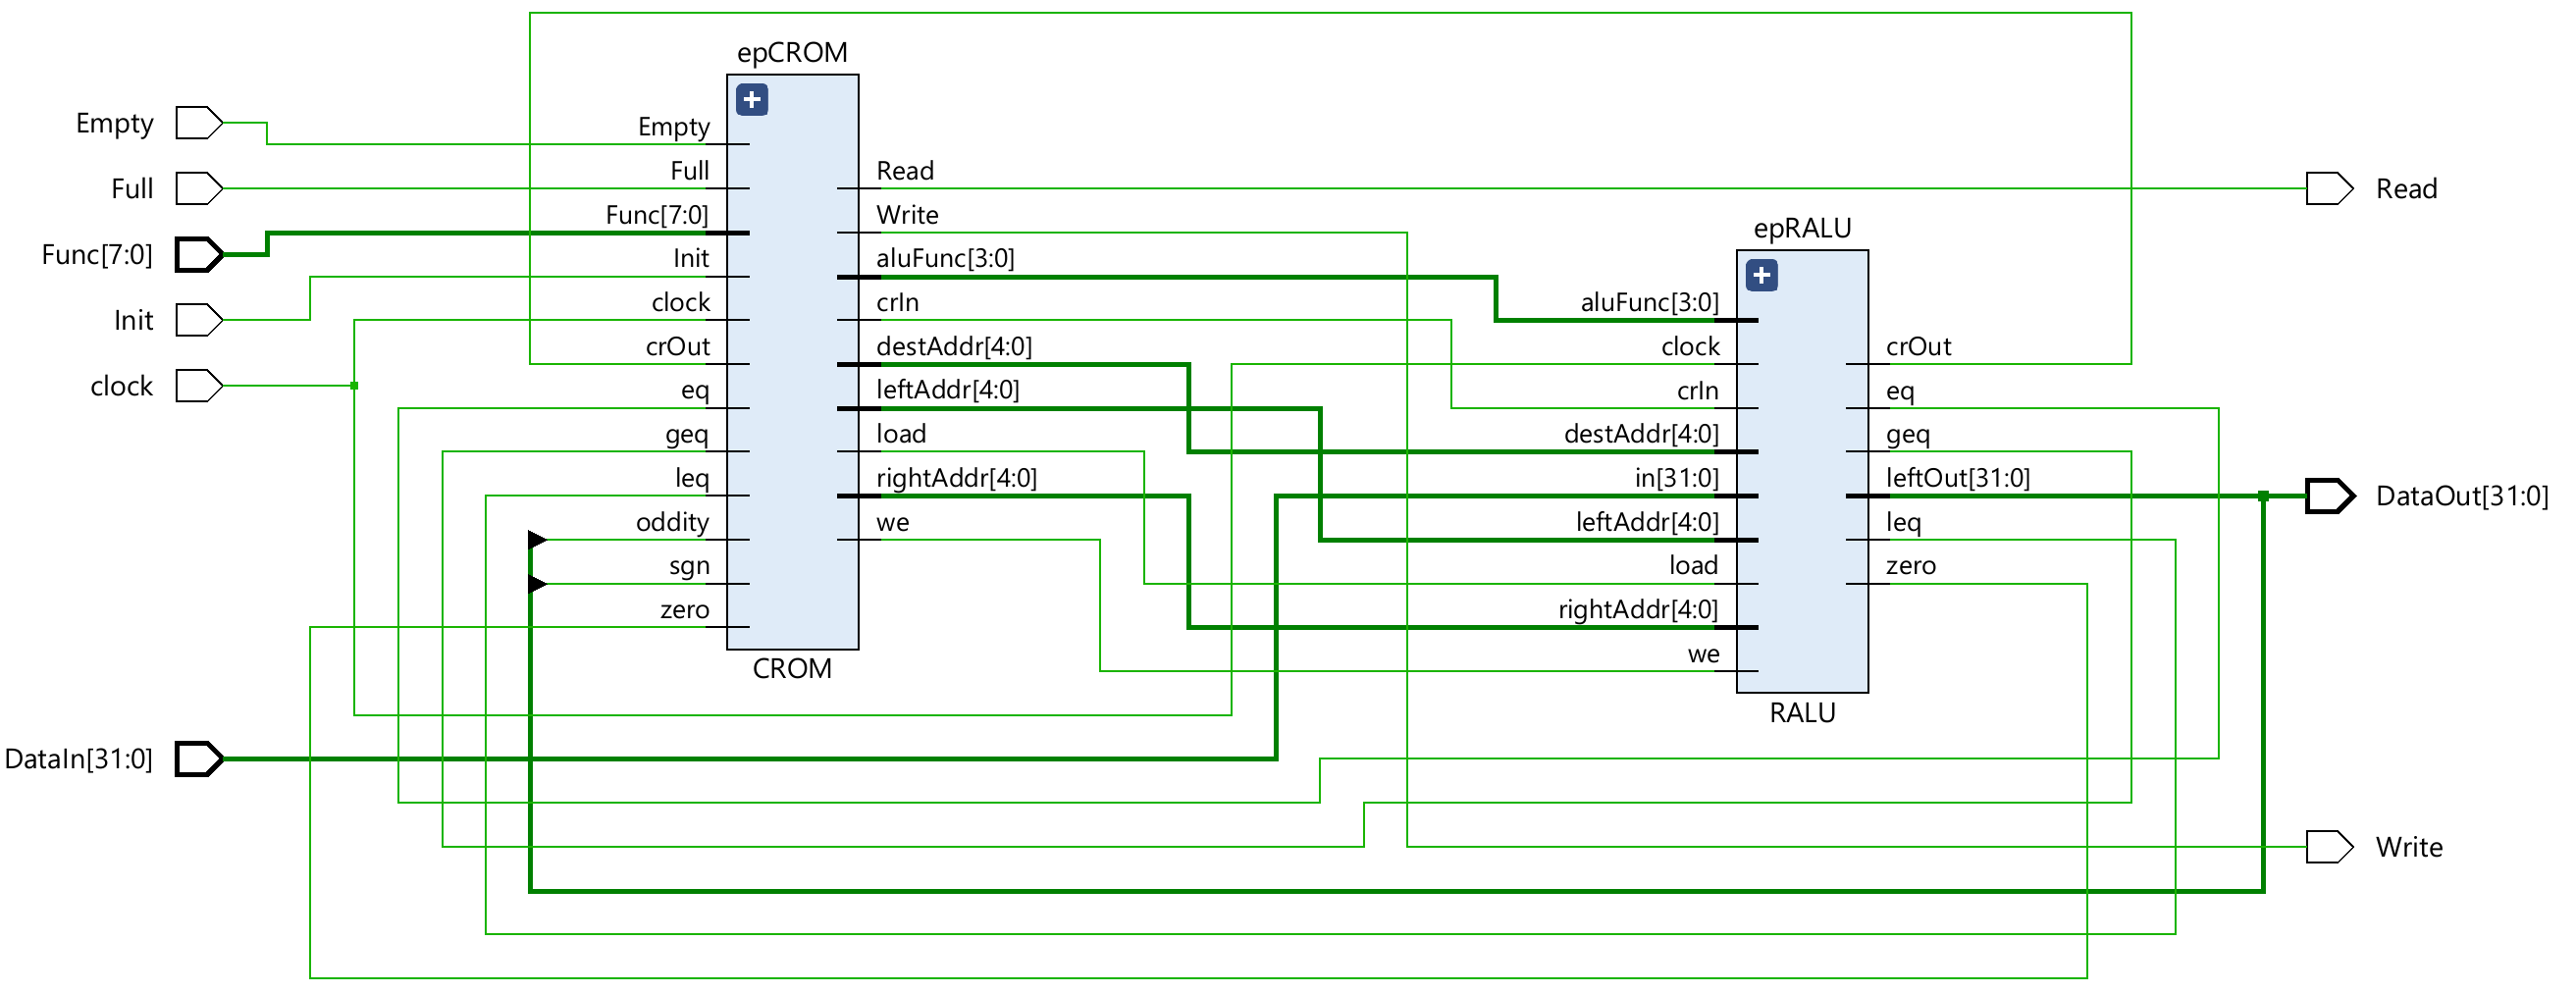
\includegraphics[width=\textwidth]{elementaryProcessor.png}
\end{center}
\vspace{0.2cm}
\begin{center}

\end{center}
\end{column}
\end{columns}
\end{frame}

\begin{frame}{RALU: Registers with ALU}
\begin{columns}
\begin{column}{0.6\textwidth}
\concept{Structure}:
\begin{itemize}
\item \textbf{Register File}: Multi-port storage
\item \textbf{ALU}: Arithmetic and logic operations
\item \textbf{Flag Generation}: Status indicators
\item \textbf{Data Paths}: Interconnection network
\end{itemize}

\vspace{0.3cm}
\concept{Flag Outputs}:
\begin{itemize}
\item \textbf{crOut}: Carry output from ALU
\item \textbf{eq}: Equal (leftOut == rightOut)
\item \textbf{leq}: Less than or equal
\item \textbf{geq}: Greater than or equal
\item \textbf{zero}: Equal to zero
\item \textbf{sgn}: Sign bit (negative)
\item \textbf{oddity}: Odd number indicator
\end{itemize}
\end{column}
\begin{column}{0.4\textwidth}
\begin{center}
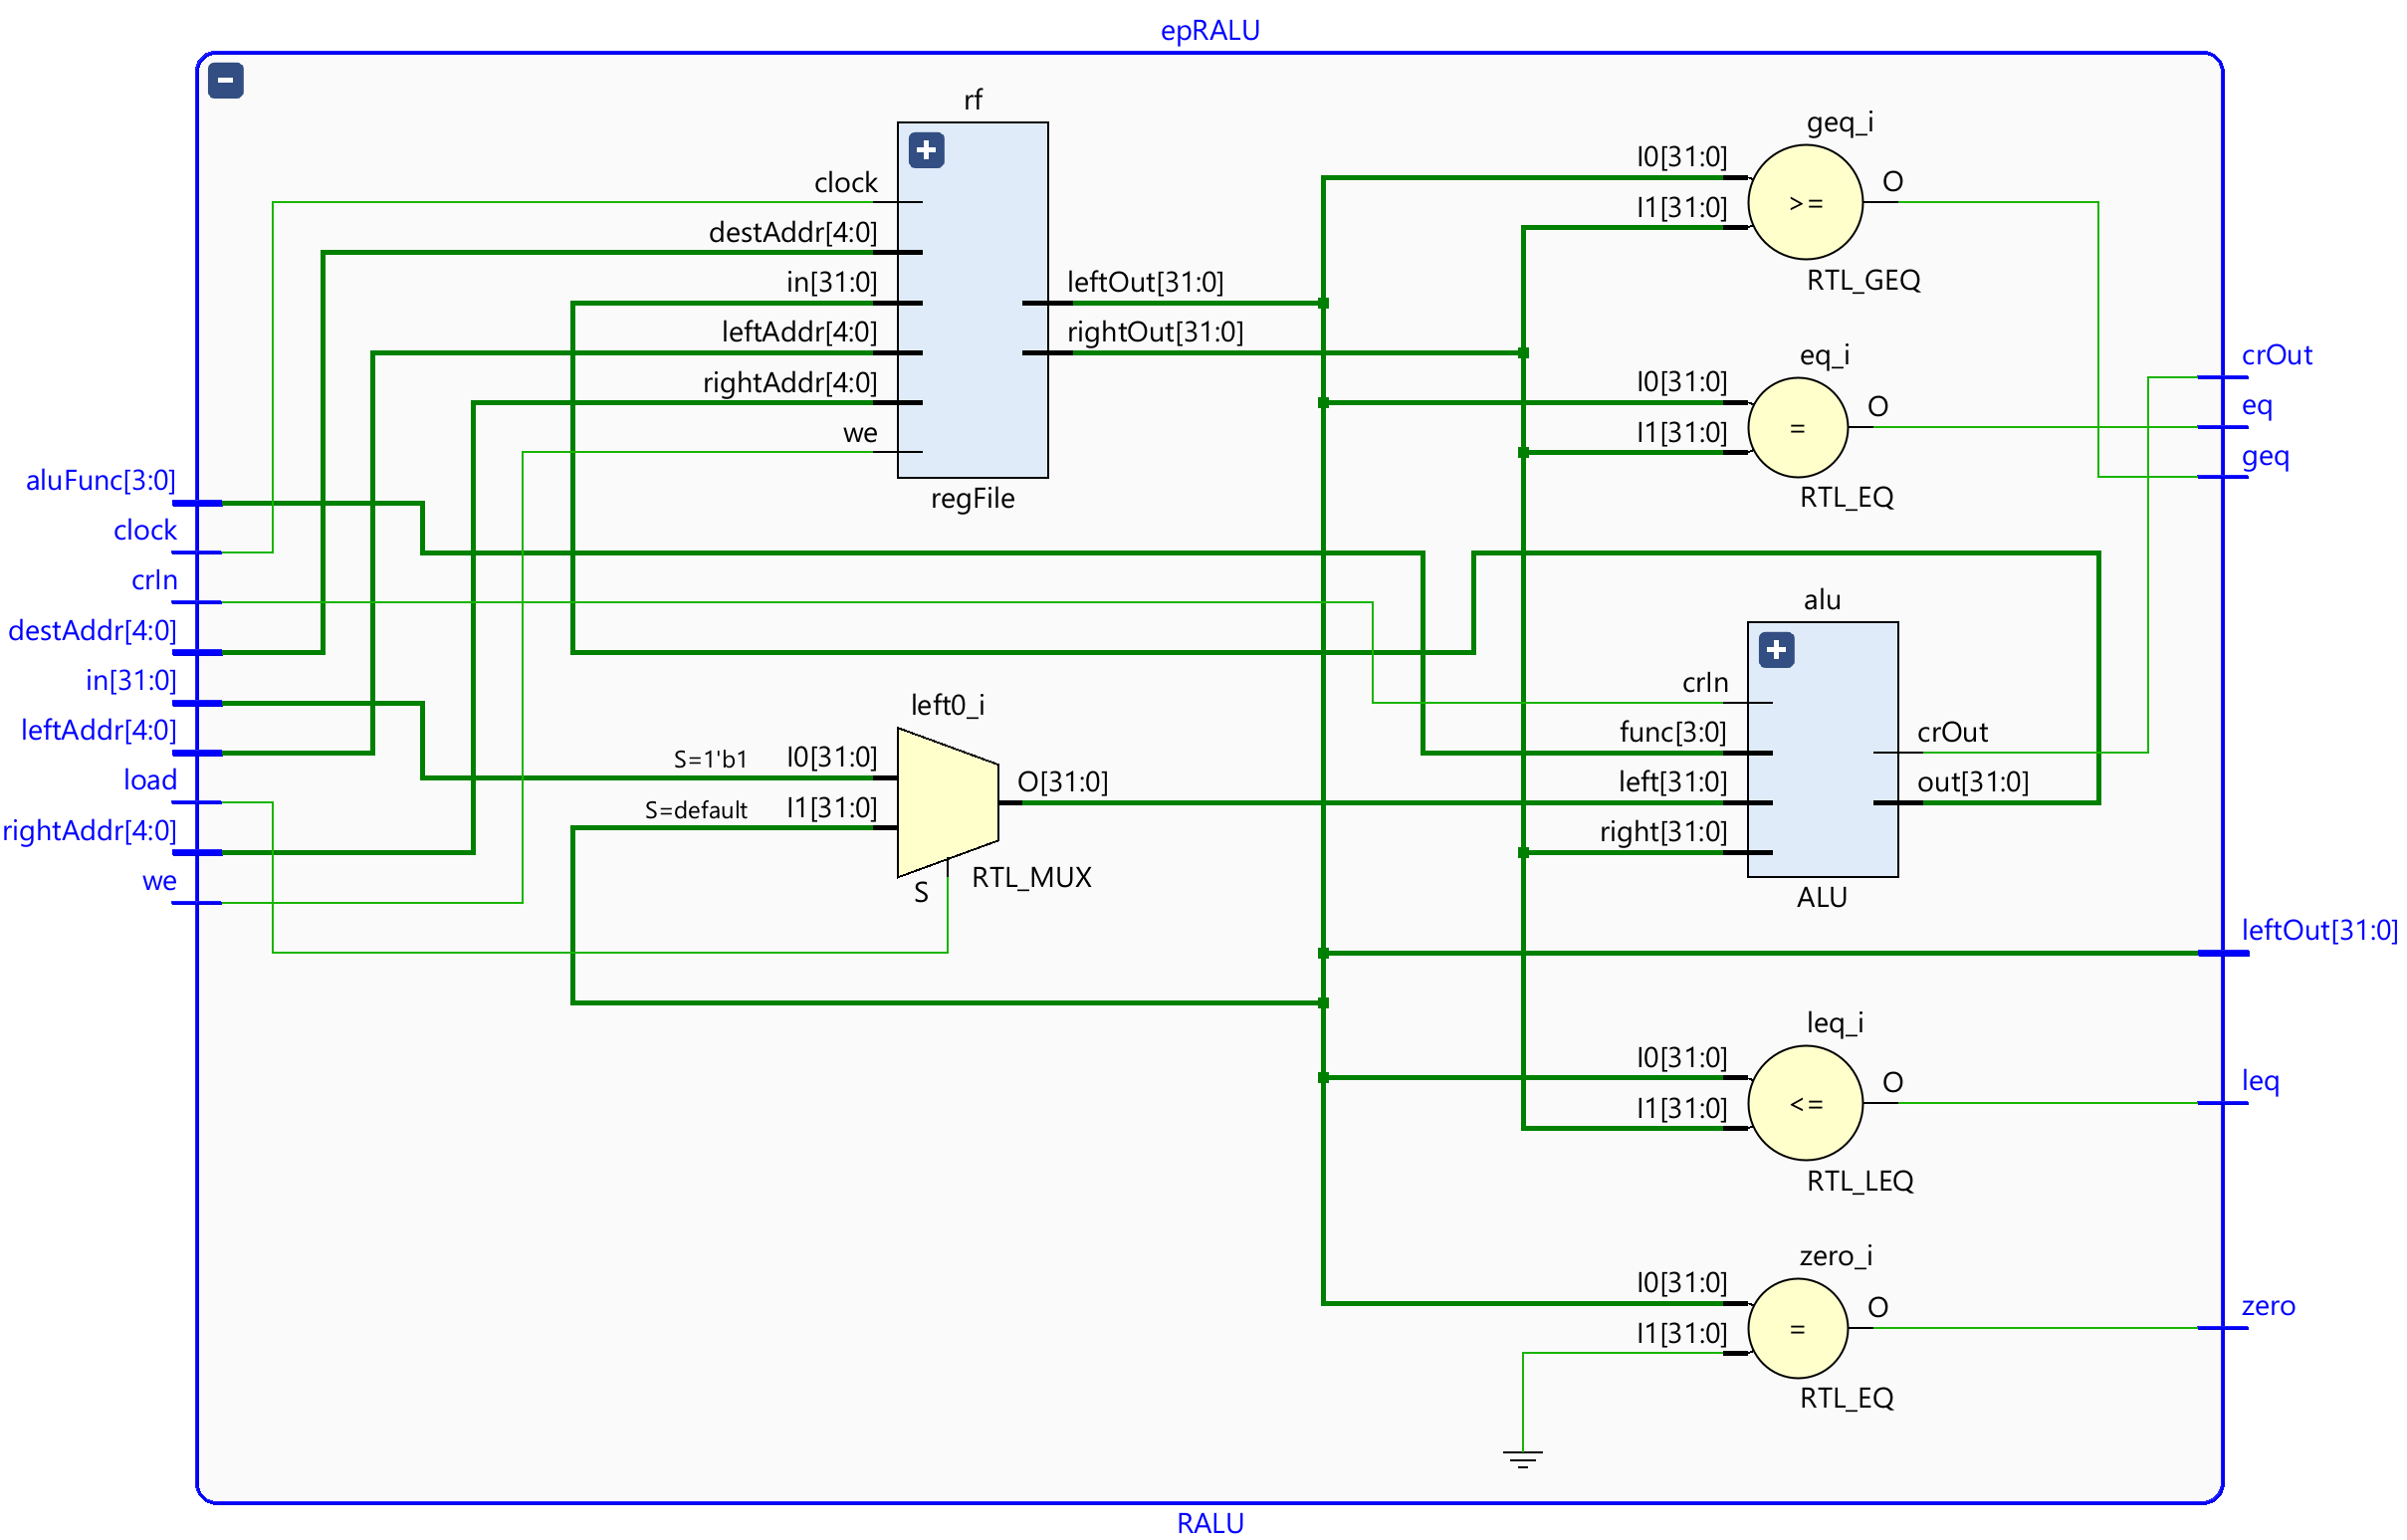
\includegraphics[width=\textwidth]{peRALU.png}
\end{center}
\concept{Characteristics}:
\begin{itemize}
\item Simple functional automaton
\item Regular, predictable structure
\item Low complexity relative to size
\item Efficient implementation
\end{itemize}
\end{column}
\end{columns}
\end{frame}

\begin{frame}{CROM: Control ROM}
\begin{columns}
\begin{column}{0.6\textwidth}
\concept{Function}:
\begin{itemize}
\item Micro-programmed control unit
\item Stores control sequences
\item Implements instruction execution
\item Provides system coordination
\end{itemize}

\vspace{0.3cm}
\concept{Components}:
\begin{itemize}
\item \textbf{ROM}: Micro-instruction storage
\item \textbf{Program Counter}: Address generation
\item \textbf{Increment Logic}: Sequential addressing
\item \textbf{Multiplexers}: Address selection
\end{itemize}

\vspace{0.3cm}
\concept{External Flags}:
\begin{itemize}
\item \textbf{Empty}: Data source empty
\item \textbf{Full}: Data receiver full
\end{itemize}
\end{column}
\begin{column}{0.4\textwidth}
\begin{center}
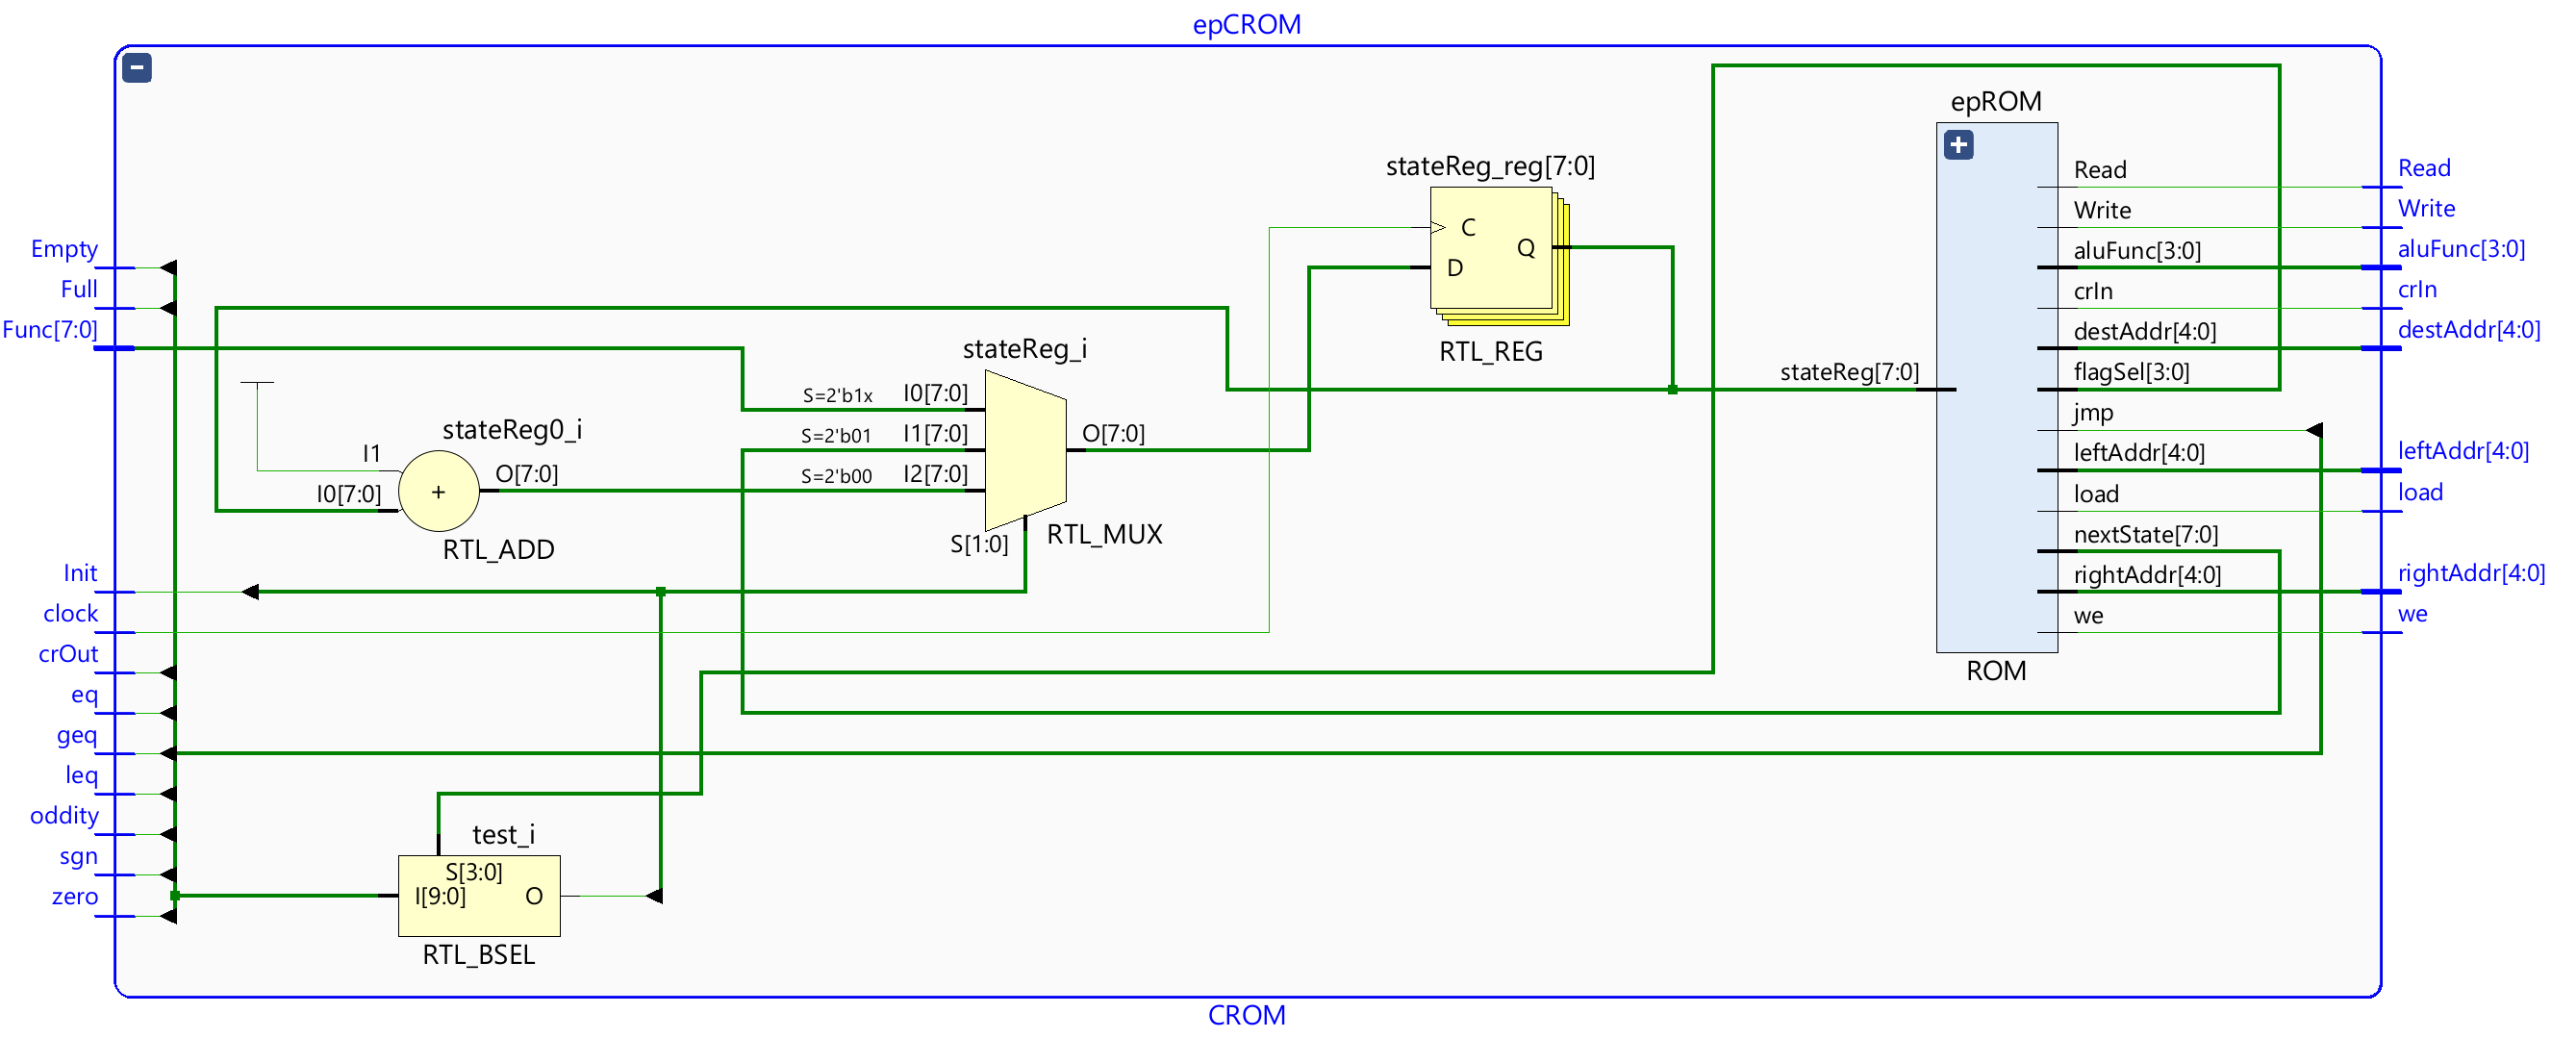
\includegraphics[width=\textwidth]{epCROM.png}
\end{center}
\concept{Characteristics}:
\begin{itemize}
\item Complex control automaton
\item High complexity relative to size
\item Flexible programming capability
\item Sophisticated behavior
\end{itemize}
\end{column}
\end{columns}
\end{frame}

% Section 4: Register File Design
\section{Register File Implementation}

\begin{frame}{Register File Architecture}
\begin{columns}
\begin{column}{0.6\textwidth}
\concept{Multi-Port Design}:
\begin{itemize}
\item Two read ports (left and right)
\item One write port
\item Simultaneous access capability
\item Independent addressing
\end{itemize}

\vspace{0.3cm}
\concept{Interface Signals}:
\begin{itemize}
\item \textbf{leftAddr}: Left read address
\item \textbf{rightAddr}: Right read address
\item \textbf{destAddr}: Write destination
\item \textbf{writeEnable}: Write control
\item \textbf{leftOut/rightOut}: Read outputs
\item \textbf{in}: Write data input
\end{itemize>
\end{column}
\begin{column}{0.4\textwidth}
\begin{center}
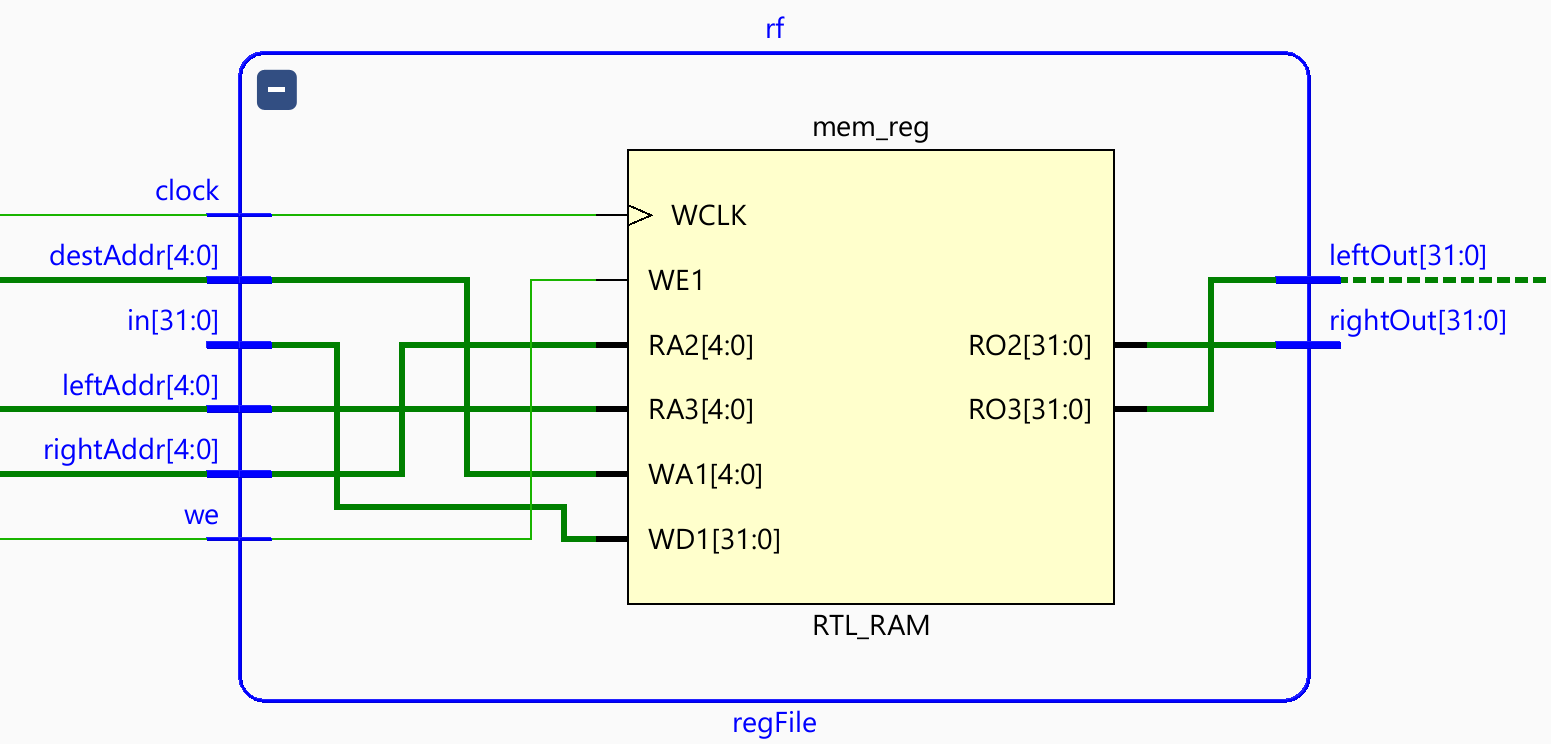
\includegraphics[width=\textwidth]{epRegFile.png}
\end{center}
\concept{Operation}:
\begin{itemize}
\item Synchronous write operation
\item Asynchronous read operation
\item Dual-port read capability
\item Register-based storage
\end{itemize>
\end{column}
\end{columns}
\end{frame}

\begin{frame}{Register File Implementation Details}
\begin{itemize}
\item \concept{Storage Structure}:
\begin{itemize}
\item Array of registers (flip-flops)
\item Addressable storage locations
\item Parallel access capability
\item Fast read/write operations
\end{itemize}
\vspace{0.5cm}
\item \concept{Access Mechanism}:
\begin{itemize}
\item Address decoders for selection
\item Multiplexers for output routing
\item Write enable gating
\item Simultaneous multi-port access
\end{itemize}
\vspace{0.3cm}
\item \concept{Design Considerations}:
\begin{itemize}
\item Area vs. performance trade-offs
\item Number of registers vs. access time
\item Power consumption optimization
\item Technology mapping considerations
\end{itemize>
\end{itemize>
\end{frame}

% Section 5: ALU Design
\section{Arithmetic Logic Unit (ALU)}

\begin{frame}{ALU Functionality}
\begin{columns}
\begin{column}{0.6\textwidth}
\concept{Supported Operations}:
\begin{itemize}
\item \textbf{BIGVAL}: Concatenation operation
\item \textbf{ADD}: Addition
\item \textbf{SUB}: Subtraction
\item \textbf{ADDCR}: Addition with carry
\item \textbf{SUBCR}: Subtraction with carry
\item \textbf{LSH}: Logical shift
\item \textbf{ASH}: Arithmetic shift
\end{itemize>

\vspace{0.3cm}
\concept{Control Interface}:
\begin{itemize}
\item \textbf{aluFunc[3:0]}: Operation selection
\item \textbf{crIn}: Carry input
\item \textbf{crOut}: Carry output flag
\end{itemize>
\end{column}
\begin{column}{0.4\textwidth}
\begin{center}
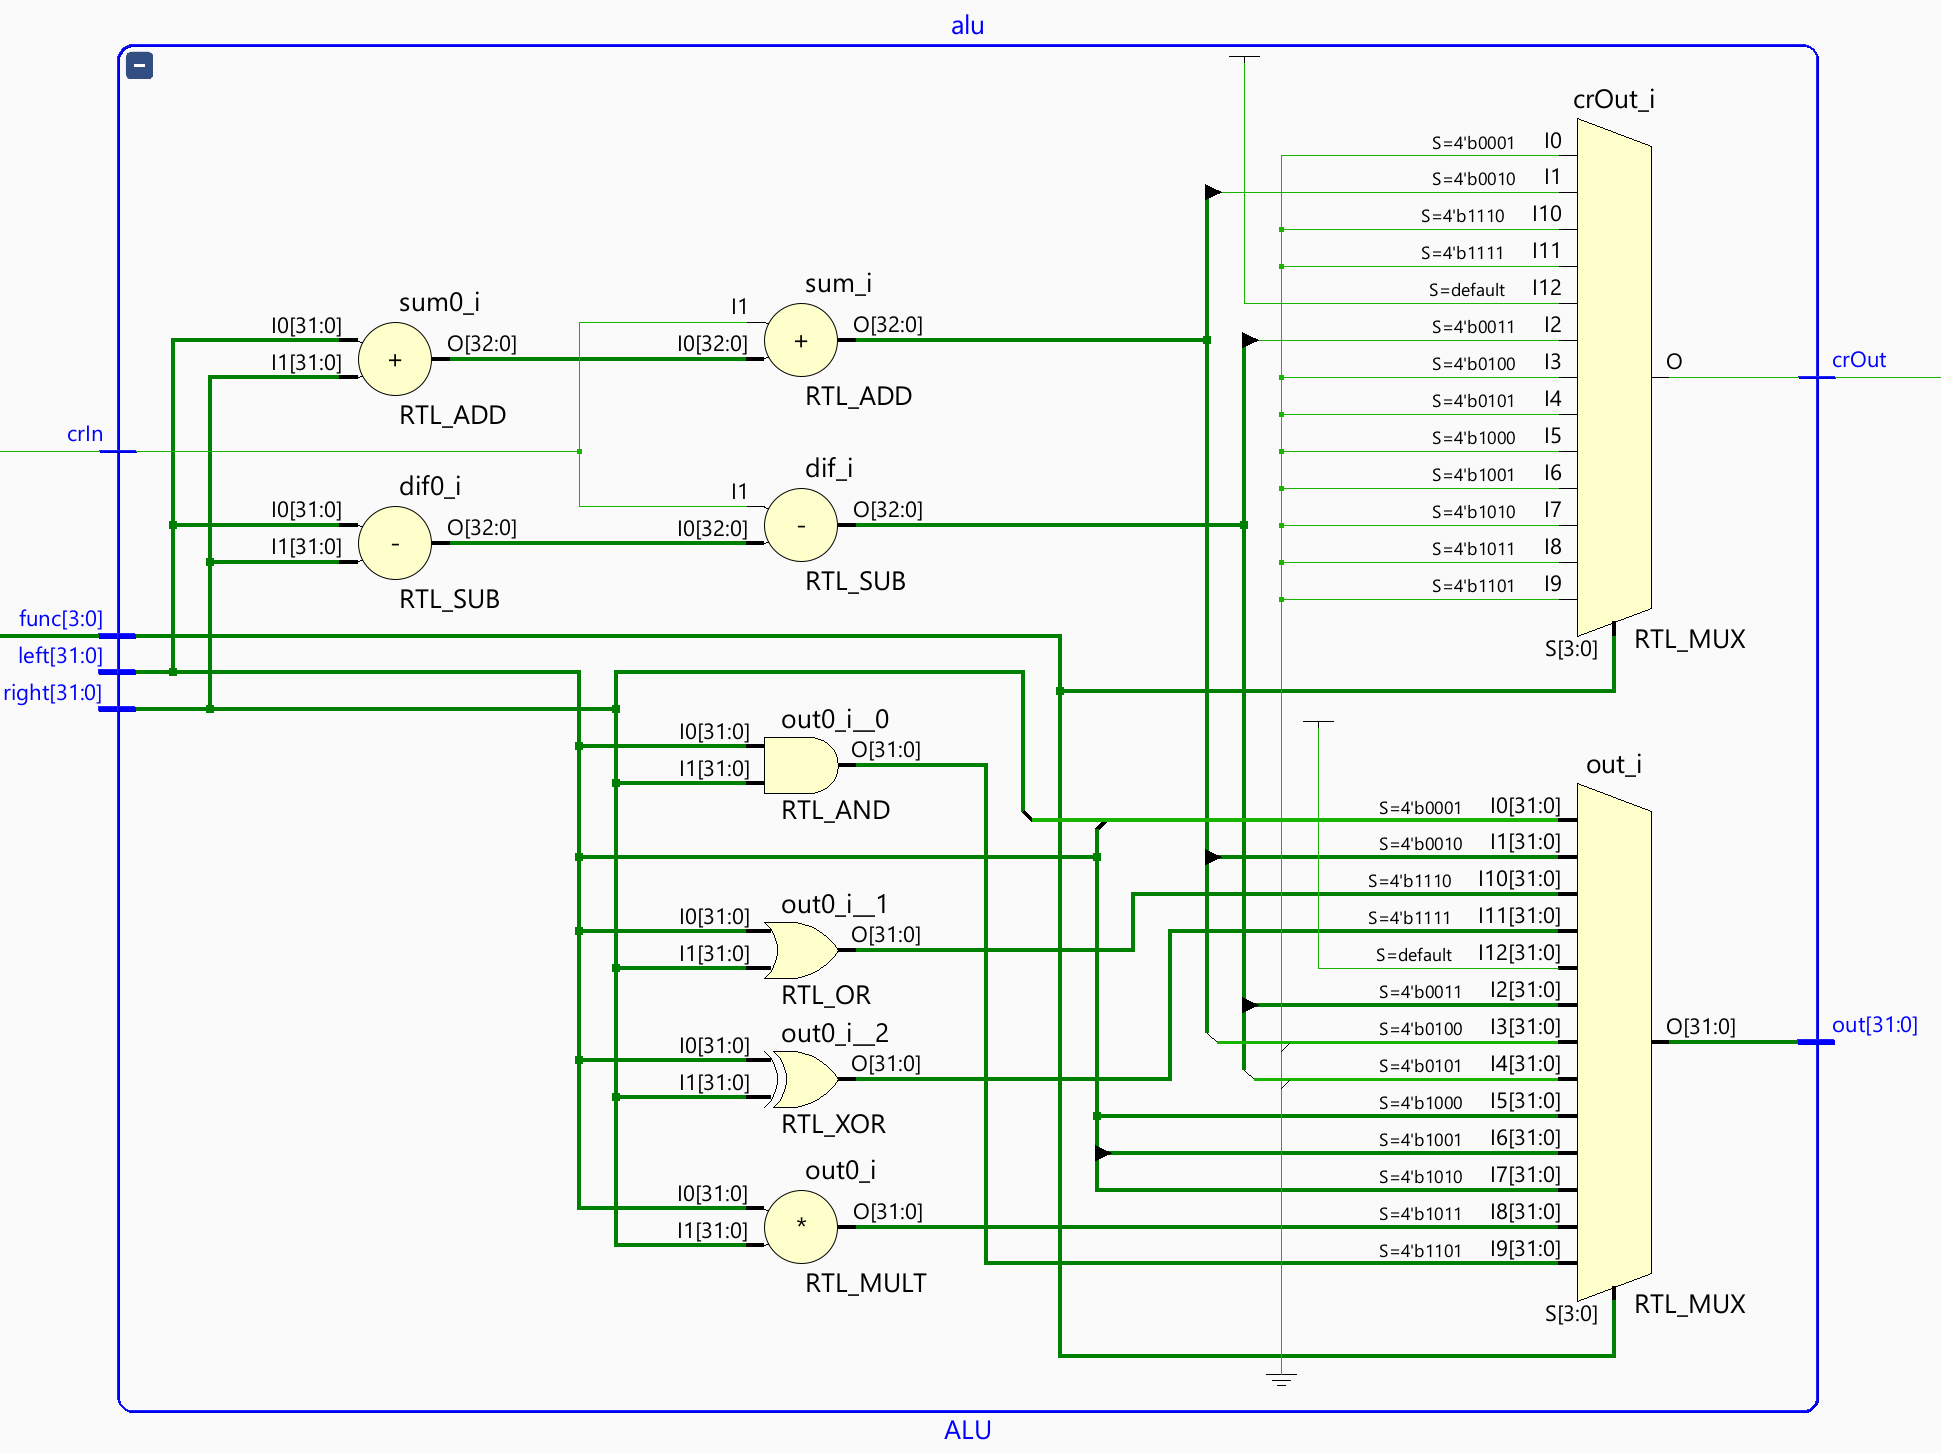
\includegraphics[width=\textwidth]{epALU.png}
\end{center}
\concept{Design Features}:
\begin{itemize}
\item Multi-function capability
\item Flag generation
\item Carry chain support
\item Efficient implementation
\end{itemize>
\end{column}
\end{columns}
\end{frame}

\begin{frame}{ALU Operation Examples}
\begin{itemize}
\item \concept{Arithmetic Operations}:
\begin{itemize}
\item \textbf{ADD}: $D(X) \leftarrow L(Y) + R(Z)$
\item \textbf{SUB}: $D(X) \leftarrow L(Y) - R(Z)$
\item \textbf{ADDCR}: Addition with carry propagation
\item \textbf{SUBCR}: Subtraction with borrow
\end{itemize>
\vspace{0.5cm}
\item \concept{Logical Operations}:
\begin{itemize}
\item \textbf{BIGVAL}: $D(X) \leftarrow \{L(Y)[15:0], R(Z)[15:0]\}$
\item Bit manipulation operations
\item Boolean logic functions
\end{itemize>
\vspace{0.3cm}
\item \concept{Shift Operations}:
\begin{itemize}
\item \textbf{LSH}: $D(X) \leftarrow \{1'b0, L(Y)[31:1]\}$
\item \textbf{ASH}: $D(X) \leftarrow \{L(Y)[31], L(Y)[31:1]\}$
\item Multiplication/division by powers of 2
\end{itemize>
\end{itemize>
\end{frame}

% Section 6: Control ROM and Micro-programming
\section{Control ROM and Micro-programming}

\begin{frame}{ROM Structure}
\begin{columns}
\begin{column}{0.6\textwidth}
\concept{Function}:
\begin{itemize}
\item Stores micro-instructions
\item Provides control sequences
\item Implements instruction execution
\item Enables programmable control
\end{itemize>

\vspace{0.3cm}
\concept{Interface}:
\begin{itemize}
\item \textbf{Address Input}: Micro-PC value
\item \textbf{Data Output}: Micro-instruction
\item \textbf{Enable Signal}: Access control
\item \textbf{Clock}: Synchronization
\end{itemize>

\vspace{0.3cm>
\concept{Content Generation}:
\begin{itemize}
\item Micro-code generator tool
\item Assembly-like programming
\item Binary encoding
\item Verification and testing
\end{itemize>
\end{column}
\begin{column}{0.4\textwidth}
\begin{center}
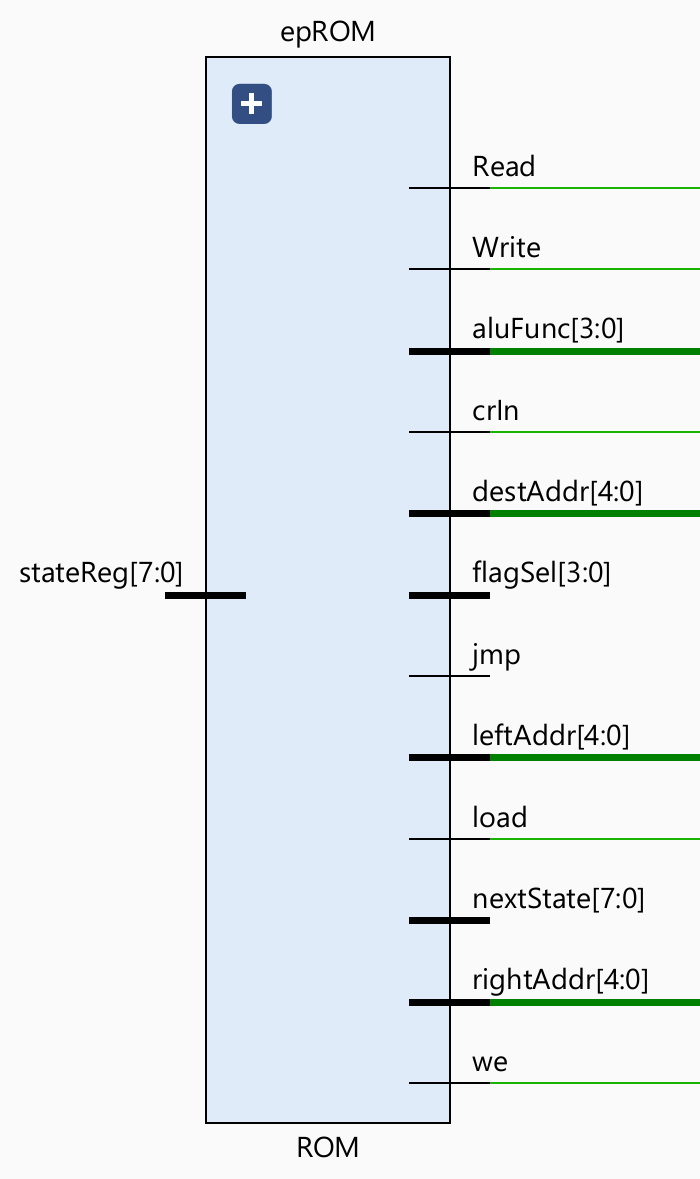
\includegraphics[width=\textwidth]{epROM.png}
\end{center}
\concept{Characteristics}:
\begin{itemize}
\item Read-only memory
\item Fast access time
\item Programmable content
\item Reliable operation
\end{itemize>
\end{column}
\end{columns}
\end{frame}

\begin{frame}{Micro-instruction Format}
\begin{itemize}
\item \concept{Control Fields} (12 fields total):
\begin{itemize}
\item \textbf{nextState[7:0]}: Next state address
\item \textbf{jmp}: Unconditional jump control
\item \textbf{flagSel[3:0]}: Conditional jump flag selection
\item \textbf{leftAddr[4:0]}: Left operand address
\item \textbf{rightAddr[4:0]}: Right operand address
\item \textbf{destAddr[4:0]}: Destination address
\end{itemize>
\vspace{0.3cm>
\item \concept{Operation Fields}:
\begin{itemize}
\item \textbf{crIn}: Carry input control
\item \textbf{load}: Data input selection
\item \textbf{we}: Write enable control
\item \textbf{aluFunc[3:0]}: ALU function selection
\end{itemize>
\end{itemize>
\end{frame}

\begin{frame}{Micro-programming Assembly Language}
\begin{itemize}
\item \concept{Jump Instructions}:
\begin{itemize}
\item \textbf{JMP(<label>)}: Unconditional jump
\item \textbf{CRJMP(<label>)}: Jump if carry
\item \textbf{ZJMP(<label>)}: Jump if zero
\item \textbf{EQJMP(<label>)}: Jump if equal
\item \textbf{EMPTYJMP(<label>)}: Jump if input empty
\item \textbf{FULLJMP(<label>)}: Jump if output full
\end{itemize>
\vspace{0.3cm>
\item \concept{Data Operations}:
\begin{itemize}
\item \textbf{L(<address>)}: Left operand selection
\item \textbf{R(<address>)}: Right operand selection
\item \textbf{D(<address>)}: Destination selection
\item \textbf{LOAD}: Load from data input
\item \textbf{WB}: Write back to register file
\end{itemize>
\vspace{0.3cm>
\item \concept{ALU Functions}:
\begin{itemize}
\item \textbf{ADD, SUB}: Arithmetic operations
\item \textbf{LSH, ASH}: Shift operations
\item \textbf{BIGVAL}: Concatenation
\end{itemize>
\end{itemize>
\end{frame}

% Section 7: Processor Operation
\section{Elementary Processor Operation}

\begin{frame}{Instruction Execution Cycle}
\begin{itemize}
\item \concept{Fetch Phase}:
\begin{itemize}
\item Retrieve micro-instruction from ROM
\item Decode control fields
\item Prepare operand addresses
\item Set up ALU function
\end{itemize>
\vspace{0.5cm>
\item \concept{Execute Phase}:
\begin{itemize}
\item Read operands from register file
\item Perform ALU operation
\item Generate status flags
\item Determine next state
\end{itemize>
\vspace{0.3cm>
\item \concept{Write-back Phase}:
\begin{itemize}
\item Store result in destination register
\item Update program counter
\item Handle conditional branches
\item Prepare for next cycle
\end{itemize>
\end{itemize>
\end{frame}

\begin{frame}{Control Flow Management}
\begin{itemize}
\item \concept{Sequential Execution}:
\begin{itemize}
\item Program counter increment
\item Linear instruction flow
\item Default operation mode
\end{itemize>
\vspace{0.5cm>
\item \concept{Conditional Branching}:
\begin{itemize}
\item Flag-based decisions
\item Multiple condition types
\item Dynamic control flow
\item Context-sensitive behavior
\end{itemize>
\vspace{0.3cm>
\item \concept{External Interface}:
\begin{itemize}
\item Data input/output coordination
\item Flow control mechanisms
\item System integration support
\item Real-time response capability
\end{itemize>
\end{itemize>
\end{frame}

% Section 8: Programming Model
\section{Programming Model and Applications}

\begin{frame}{Programming Paradigm}
\begin{itemize}
\item \concept{Micro-programming Level}:
\begin{itemize}
\item Low-level control specification
\item Hardware-oriented programming
\item Cycle-by-cycle control
\item Maximum flexibility
\end{itemize>
\vspace{0.5cm>
\item \concept{Assembly Language Interface}:
\begin{itemize>
\item Human-readable mnemonics
\item Label-based addressing
\item Structured programming support
\item Debugging capabilities
\end{itemize>
\vspace{0.3cm>
\item \concept{Application Areas}:
\begin{itemize>
\item Digital signal processing
\item Control system implementation
\item Educational processor design
\item Embedded system controllers
\end{itemize>
\end{itemize>
\end{frame}

\begin{frame}{Context-Free Language Processing}
\begin{itemize>
\item \concept{Enhanced Capabilities}:
\begin{itemize>
\item Stack-like behavior simulation
\item Nested structure processing
\item Recursive pattern recognition
\item Context-free grammar parsing
\end{itemize>
\vspace{0.5cm>
\item \concept{Example Applications}:
\begin{itemize>
\item Expression evaluation
\item Parentheses matching
\item Compiler front-end processing
\item Syntax analysis
\end{itemize>
\vspace{0.3cm>
\item \concept{Advantages over 2-OS}:
\begin{itemize>
\item Higher computational power
\item More complex language recognition
\item Enhanced problem-solving capability
\item Greater programming flexibility
\end{itemize>
\end{itemize>
\end{frame}

% Section 9: Design Considerations
\section{Design Considerations and Trade-offs}

\begin{frame}{Performance Optimization}
\begin{itemize>
\item \concept{Speed Considerations}:
\begin{itemize>
\item Clock frequency limitations
\item Critical path analysis
\item Pipeline potential
\item Instruction throughput
\end{itemize>
\vspace{0.5cm>
\item \concept{Area Optimization}:
\begin{itemize>
\item Register file size
\item ROM capacity
\item ALU complexity
\item Control logic overhead
\end{itemize>
\vspace{0.3cm>
\item \concept{Power Management}:
\begin{itemize>
\item Clock gating opportunities
\item Unused resource shutdown
\item Dynamic voltage scaling
\item Activity-based optimization
\end{itemize>
\end{itemize>
\end{frame}

\begin{frame}{Scalability and Extensions}
\begin{itemize>
\item \concept{Architectural Extensions}:
\begin{itemize>
\item Larger register files
\item Enhanced ALU functions
\item Multiple execution units
\item Cache memory integration
\end{itemize>
\vspace{0.5cm>
\item \concept{System Integration}:
\begin{itemize>
\item Multi-processor configurations
\item Shared memory systems
\item Communication interfaces
\item Interrupt handling
\end{itemize>
\vspace{0.3cm>
\item \concept{Technology Adaptation}:
\begin{itemize>
\item FPGA implementation
\item ASIC optimization
\item Advanced process nodes
\item Emerging technologies
\end{itemize>
\end{itemize>
\end{frame}

% Section 10: Summary
\section{Chapter Summary}

\begin{frame}{Key Concepts Review}
\begin{itemize>
\item \concept{Third-Order Systems (3-OS)}:
\begin{itemize>
\item Third feedback loop enables complex computation
\item Context-free language processing capability
\item Elementary processor implementation
\end{itemize>
\vspace{0.3cm>
\item \concept{Processor Architecture}:
\begin{itemize>
\item RALU: Simple functional automaton
\item CROM: Complex control automaton
\item Micro-programmed control approach
\end{itemize>
\vspace{0.3cm>
\item \concept{Implementation Components}:
\begin{itemize>
\item Multi-port register file
\item Arithmetic logic unit
\item Control ROM and micro-programming
\end{itemize>
\end{itemize>
\end{frame}

\begin{frame}{Design Principles}
\begin{itemize>
\item \concept{Separation of Concerns}:
\begin{itemize>
\item Data processing (RALU)
\item Control sequencing (CROM)
\item Clear interface definition
\end{itemize>
\vspace{0.3cm>
\item \concept{Programmability}:
\begin{itemize>
\item Micro-instruction format
\item Assembly language interface
\item Flexible control sequences
\end{itemize>
\vspace{0.3cm>
\item \concept{Scalability}:
\begin{itemize>
\item Modular design approach
\item Extensible architecture
\item Technology independence
\end{itemize>
\end{itemize>
\end{frame}

\begin{frame}{Computational Significance}
\begin{itemize>
\item \concept{Language Recognition Hierarchy}:
\begin{itemize>
\item 0-OS: No language recognition
\item 1-OS: Simple pattern matching
\item 2-OS: Regular languages (Type 3)
\item 3-OS: Context-free languages (Type 2)
\end{itemize>
\vspace{0.3cm>
\item \concept{Practical Applications}:
\begin{itemize>
\item Compiler design and implementation
\item Digital signal processing
\item Control system applications
\item Educational processor design
\end{itemize>
\vspace{0.3cm>
\item \concept{Foundation for Advanced Systems}:
\begin{itemize>
\item Modern processor architectures
\item Multi-core systems
\item Specialized accelerators
\item Embedded controllers
\end{itemize>
\end{itemize>
\end{frame}

% Questions slide
\begin{frame}{Questions and Discussion}
\begin{center}
\Large
Questions?

\vspace{1cm>

\normalsize
\textbf{Discussion Topics:}
\begin{itemize>
\item How does the third feedback loop enable context-free language processing?
\item What are the advantages of micro-programmed control?
\item How do RALU and CROM complement each other in processor design?
\item What role do elementary processors play in modern computer architecture?
\end{itemize>

\vspace{0.5cm>
\textbf{Conclusion:} Order-based approach provides systematic framework for understanding digital system complexity and computational capabilities.
\end{center}
\end{frame}

\end{document>

